\section{Monte Carlo via Cadeias de Markov (MCMC)}\label{mcmc}

Como alternativa ao método SIR dentro do conjunto das aproximações estocásticas, a integração via Monte Carlo em cadeias de Markov (MCMC) possui como ideia central construir cadeias de Markov, para cada variável aleatória de interesse, da qual seja possível gerar amostras e cuja distribuição limite seja estacionária e dada pela distribuição da própria variável (Migon \textit{et al.}, 2014)\cite{MiGaLou2014}. Uma cadeia de Markov é todo modelo estocástico que descreve uma sequência de eventos tal que a probabilidade de cada evento depende exclusivamente do estado atingido no evento anterior. Como grande vantagem em relação aos métodos de aproximação com quadraturas e ao SIR, o MCMC pode ser facilmente aplicado a problemas de alta dimensionalidade, inclusive quando se deseja gerar de vetores ou mesmo matrizes aleatórias.

Sejam $Y_1, \ldots, Y_p$ variáveis aleatórias com densidade conjunta $p(\bm{y}) = p(y_1, \ldots, y_p)$ definidas no espaço $\mathcal{Y} \subseteq \mathbb{R}^p$. Suponha que existe uma cadeia de Markov homogênea, irredutível e aperiódica com espaço de estados $\mathcal{Y}$ e distribuição estacionária $p(\bm{y})$. Seja $q(\bm{y}, \bm{z})$ o \textit{núcleo de transição da cadeia}, ou seja, $q(\bm{y}, \cdot)$ define uma distribuição condicional que governa as transições a partir do estado $\bm{y}$. Em outras palavras, a cadeia possui probabilidades de transição invariantes no tempo, na qual cada estado pode ser atingido a partir de qualquer outro em um número finito de iterações e sem haver estados absorventes. Assim, dado qualquer estado inicial, é possível gerar uma trajetória para a cadeia que convergirá para $p(\bm{y})$ para um número suficientemente grande de iterações. Construída a cadeia de Markov, é possível realizar uma simulação de Monte Carlo dos valores de $p$, por isso o nome MCMC.

Há vários algoritmos na literatura que permitem construir uma cadeia de Markov com distribuição limite estacionária. Neste trabalho, será usado o algoritmo de Metropolis-Hastings (Metropolis \textit{et al.}, 1953\cite{Metrop1953}; Hastings, 1970\cite{Hastin1970}), aqui abreviado por MH. Assim como o método SIR, o algoritmo MH também é baseado no uso de uma distribuição auxiliar ou proposta, aqui denotada por $q(\bm{y}, \bm{z})$. Assumindo-se que na interação $j$, $j = 1, \ldots, k$ a cadeia está no estado $\bm{y}^{(j)}$, a posição da mesma na iteração $j + 1$, denotada por $\bm{y}^{(j + 1)}$, será dada após:
\begin{itemize}
	\item Propor uma transição ou movimento para $\bm{y}^*$, onde $\bm{y}^*$ é gerada de $q(\bm{y}^{(j)}, \cdot)$, a distribuição proposta;
	\item Aceitar a transição proposta com probabilidade
	\begin{equation}\label{eq:mh_tranprob}
	\rho(\bm{y}^{(j)}, \bm{y}^*) = \min\left(1, \dfrac{p(\bm{y}^*) / q(\bm{y}^{(j)}, \bm{y}^*)}{p(\bm{y}^{(j)}) / q(\bm{y}^*, \bm{y}^{(j)})}\right)
	\end{equation}
	e neste caso atribuir $\bm{y}^{(j + 1)} = \bm{y}^*$ ou rejeitar a transição proposta e atribuir $\bm{y}^{(j + 1)} = \bm{y}^{(j)}$, com probabilidade $1 - \rho(\bm{y}^{(j)}, \bm{y}^*)$.
\end{itemize}

Para decidir sobre a aceitação ou não de $\bm{y}^*$ quando amostrada a cada passo $j$, gere uma amostra $u_1, \ldots, u_k$, onde $k$ é o total de iterações prefixadas, da distribuição uniforme padrão $U(0,1)$, independentemente de $\bm{y}^*$. Se a probabilidade de aceitação $\rho(\bm{y}^{(j)}, \bm{y}^*)$ for maior do que ou igual a $u_j$, então a transição proposta é aceita. Do contrário, ela é rejeitada.

Note ainda que se a distribuição proposta $q$ é simétrica, pode-se reescrever $\rho(\bm{y}^{(j)}, \bm{y}^*)$ em \eqref{eq:mh_tranprob} como o mínimo entre o valor unitário e a razão $p(\bm{y}^*)/p(\bm{y^{(j)}})$, simplificando o cálculo desta probabilidade. Após gerar uma amostra muito grande da variável de interesse, a inferência sobre a mesma pode ser feita assim como no SIR e em qualquer método de Monte Carlo, aproximando (por exemplo) a média populacional pela média amostral dos valores da cadeia.

\begin{figure}[t]%
	\centering
	\subfloat[Histograma de $\mu$]{{
			\label{fig:mu_mh_500}
			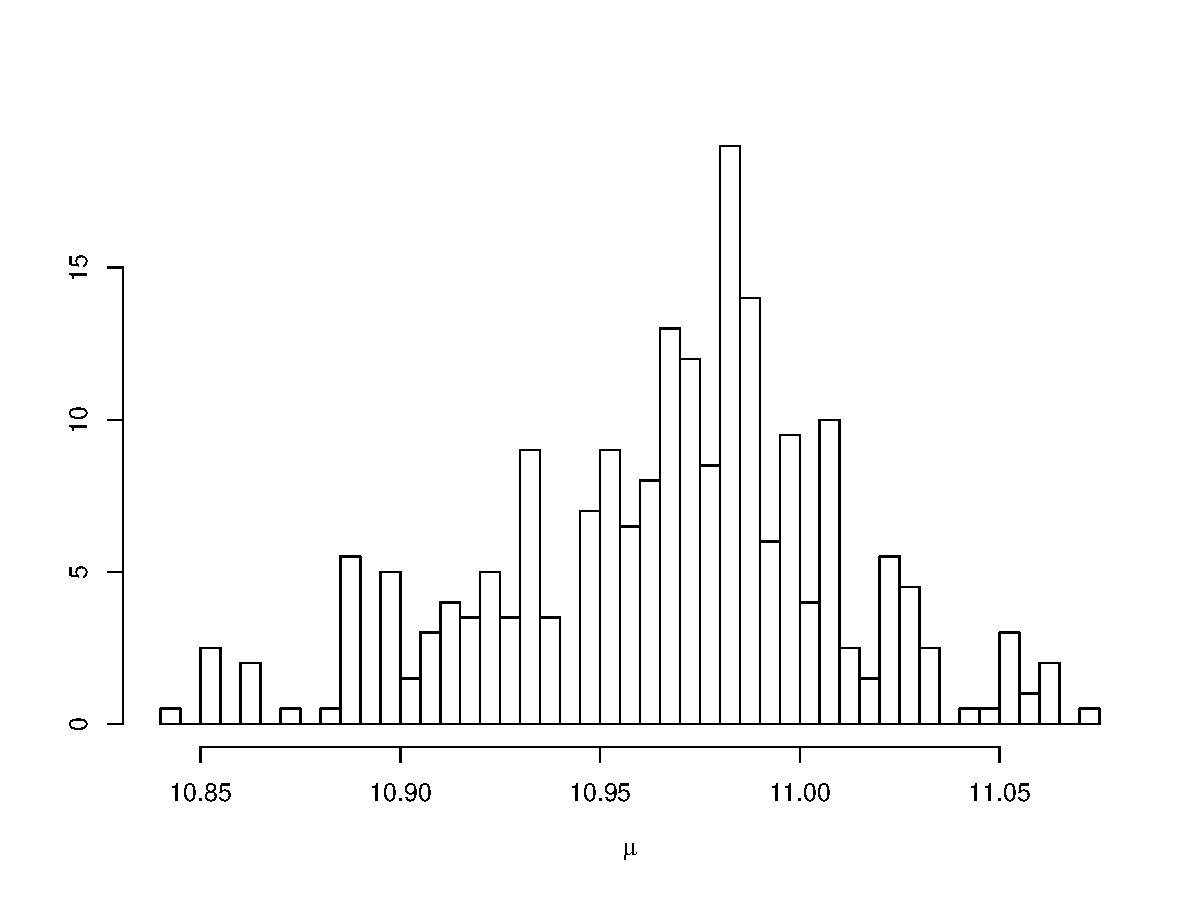
\includegraphics[scale=0.4]{figuras/mu_mh_500.pdf}}}%
	\qquad
	\subfloat[Histograma de $\sigma^2$]{{
			\label{fig:s2_mh_500}
			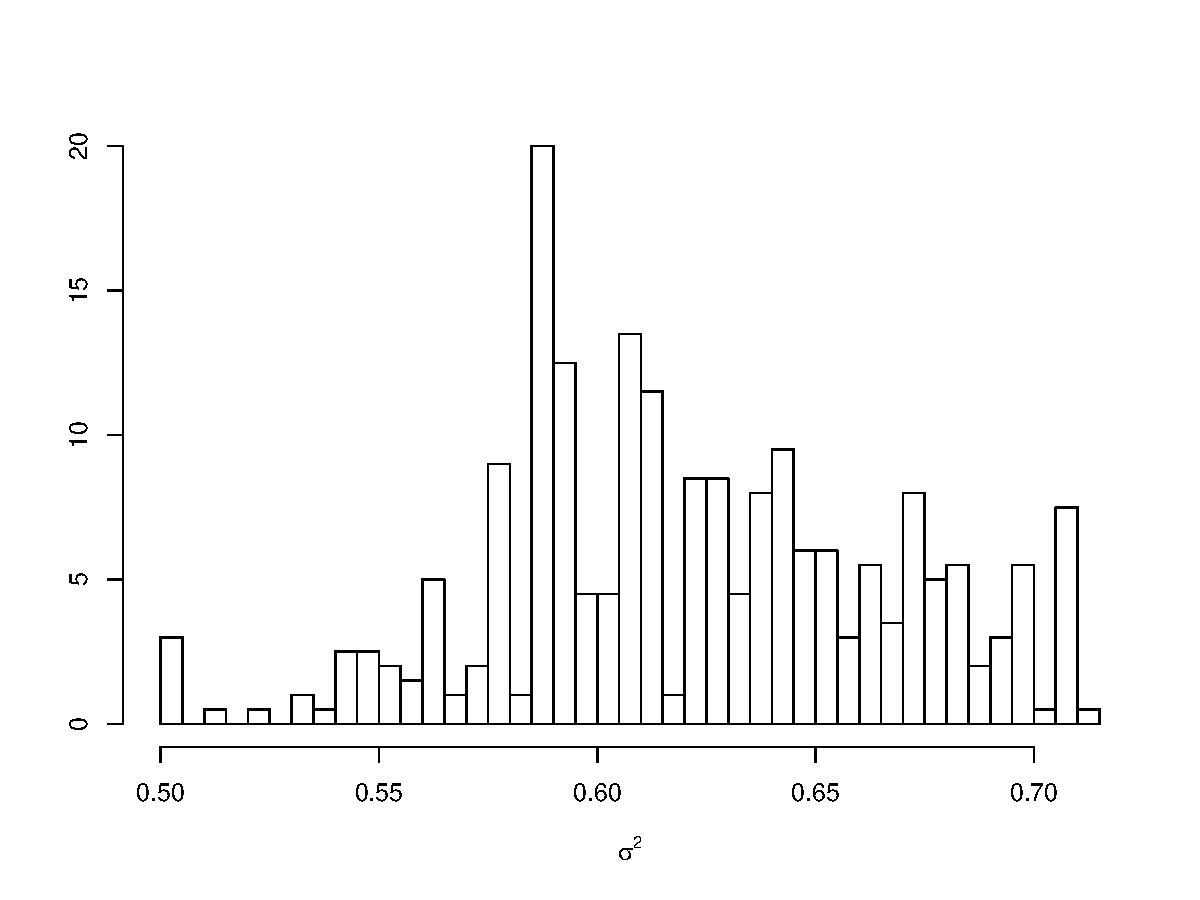
\includegraphics[scale=0.4]{figuras/s2_mh_500.pdf}}}%
	\subfloat[Histograma de $\nu$]{{
			\label{fig:nu_mh_500}
			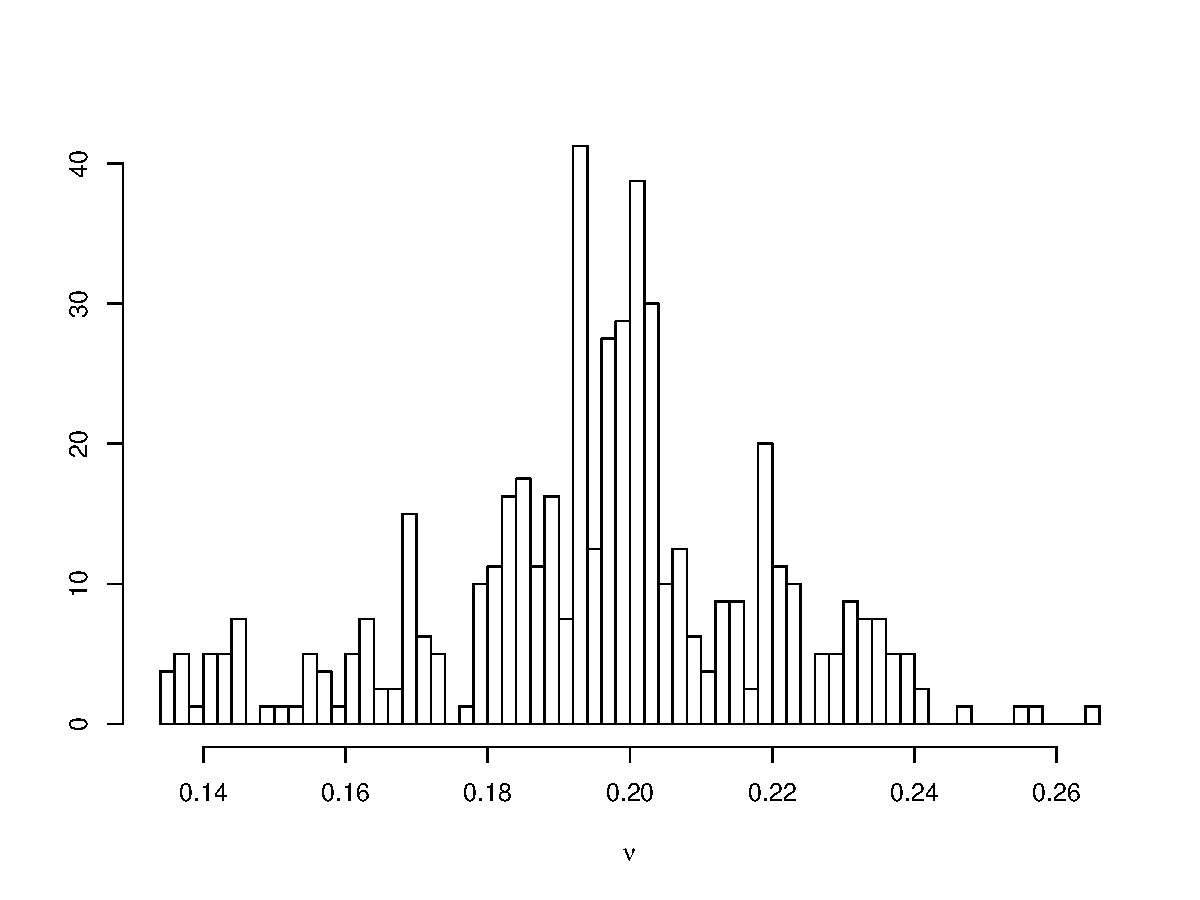
\includegraphics[scale=0.4]{figuras/nu_mh_500.pdf}}}%
	\caption{Histograma das densidades \textit{a posteriori} marginais pelo método MCMC--MH, $k = 500$}%
\end{figure}

\begin{figure}[t]%
	\centering
	\subfloat[Histograma de $\mu$]{{
			\label{fig:mu_mh_5000}
			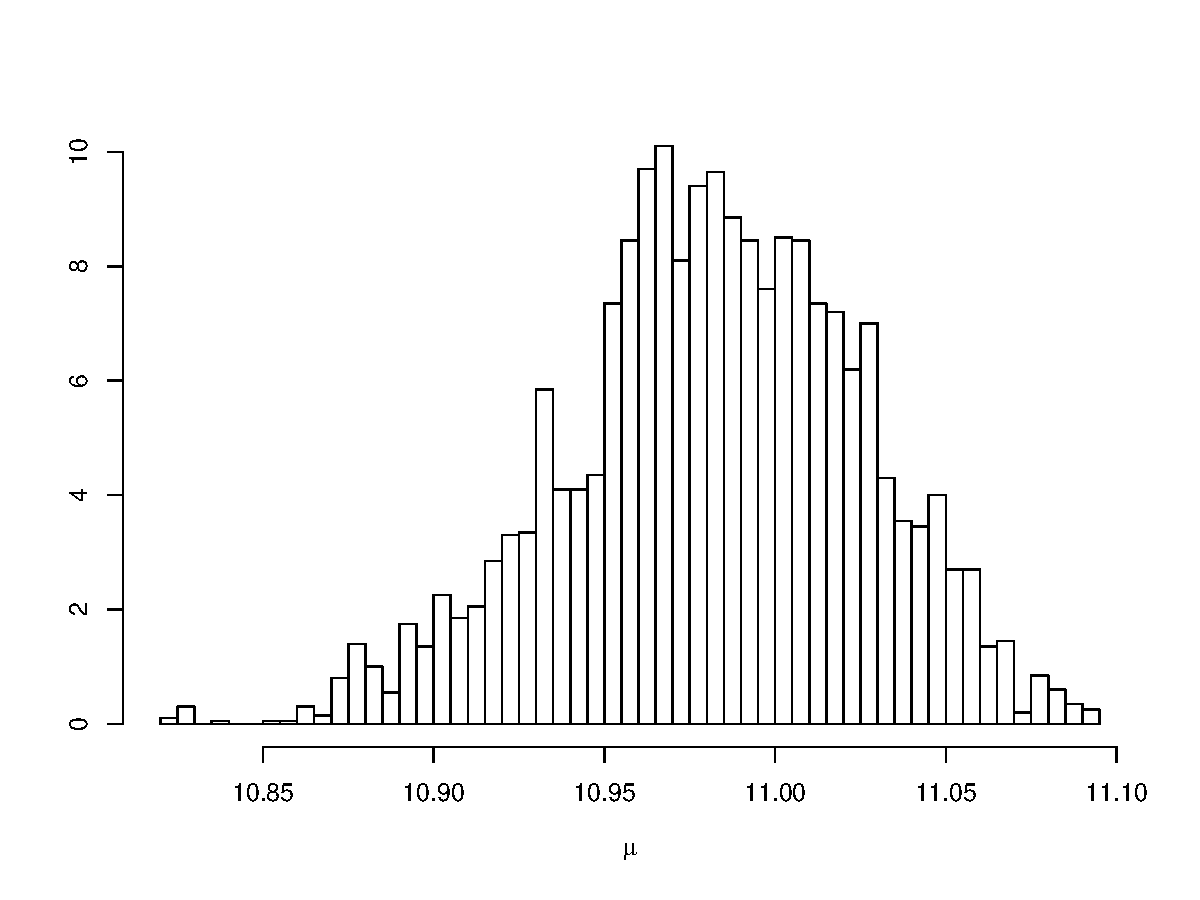
\includegraphics[scale=0.4]{figuras/mu_mh_5000.pdf}}}%
	\qquad
	\subfloat[Histograma de $\sigma^2$]{{
			\label{fig:s2_mh_5000}
			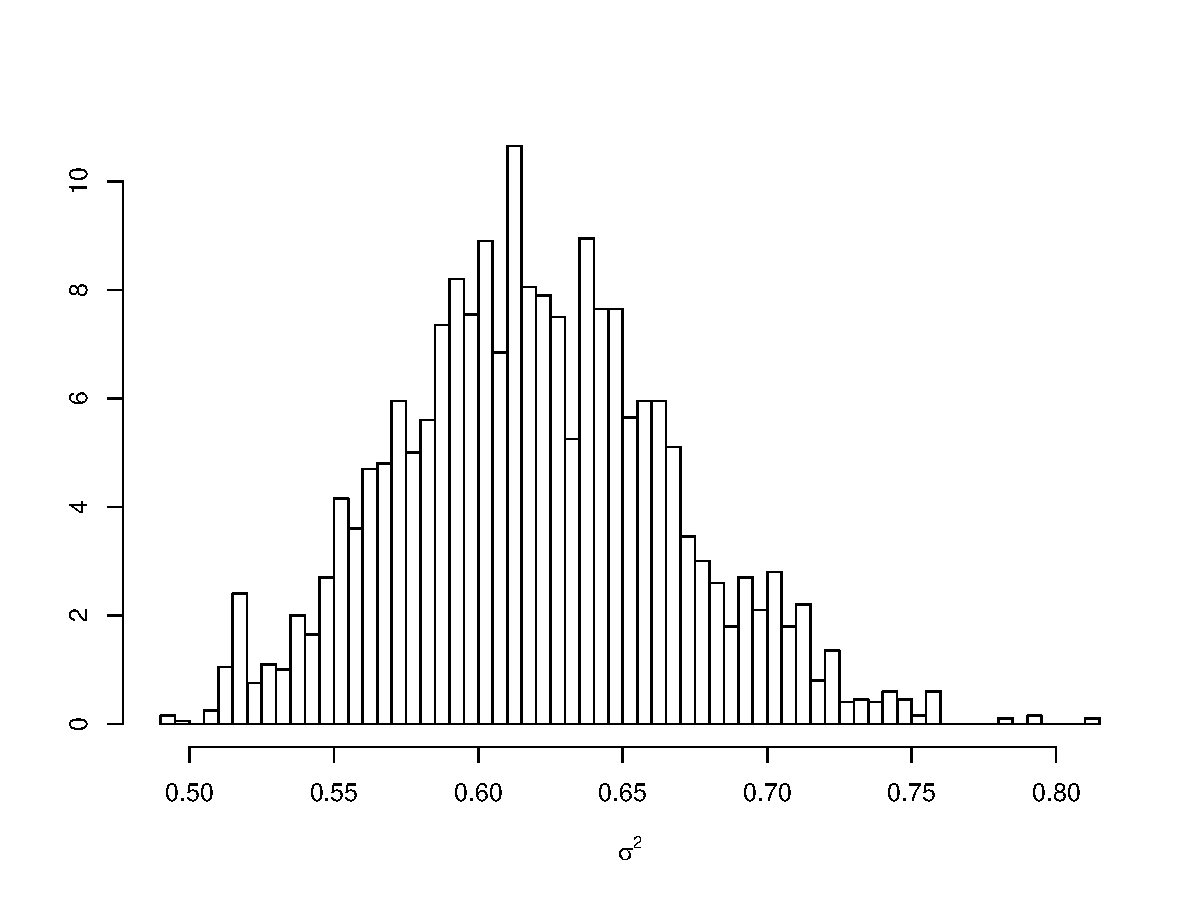
\includegraphics[scale=0.4]{figuras/s2_mh_5000.pdf}}}%
	\subfloat[Histograma de $\nu$]{{
			\label{fig:nu_mh_5000}
			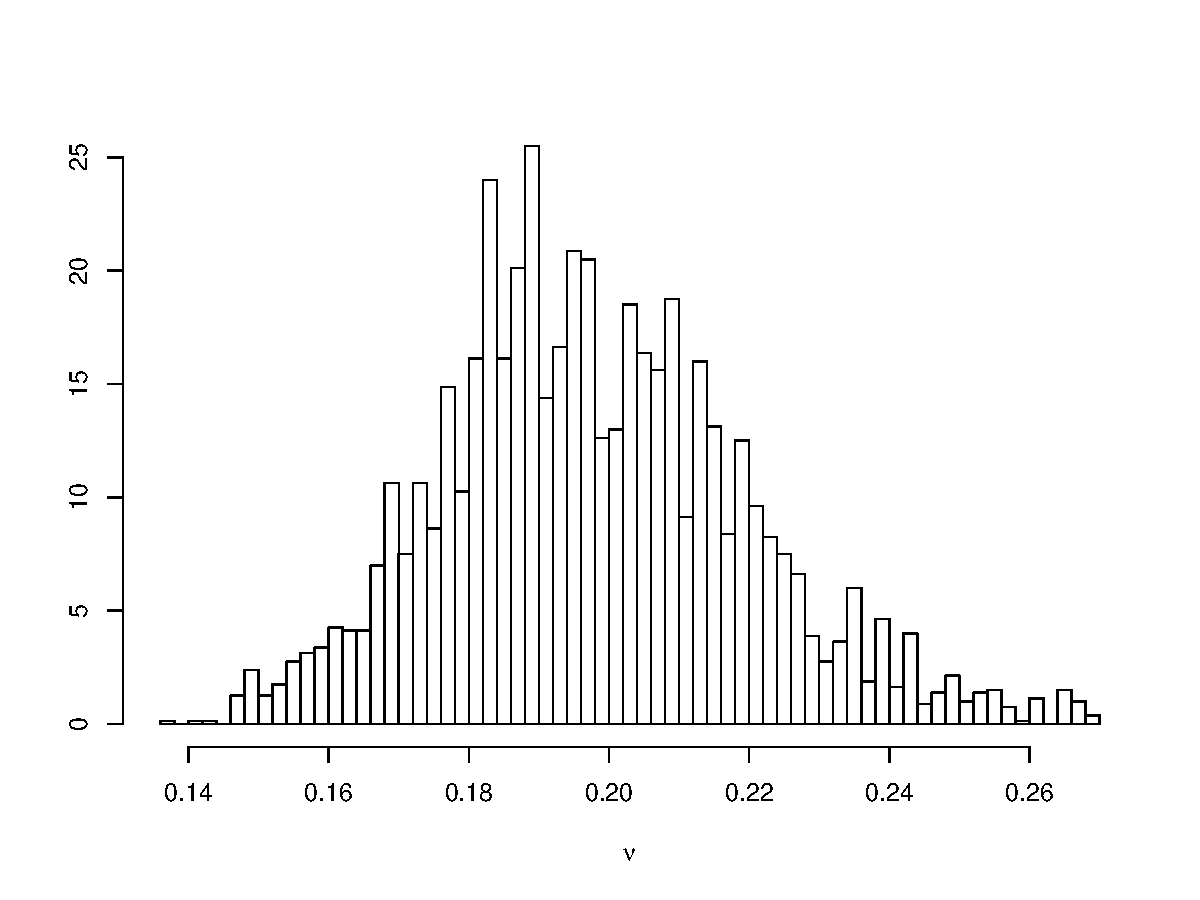
\includegraphics[scale=0.4]{figuras/nu_mh_5000.pdf}}}%
	\caption{Histograma das densidades \textit{a posteriori} marginais pela método MCMC--MH, $k = 5000$}%
\end{figure}

\begin{figure}[t]%
	\centering
	\subfloat[Histograma de $\mu$]{{
			\label{fig:mu_mh_50000}
			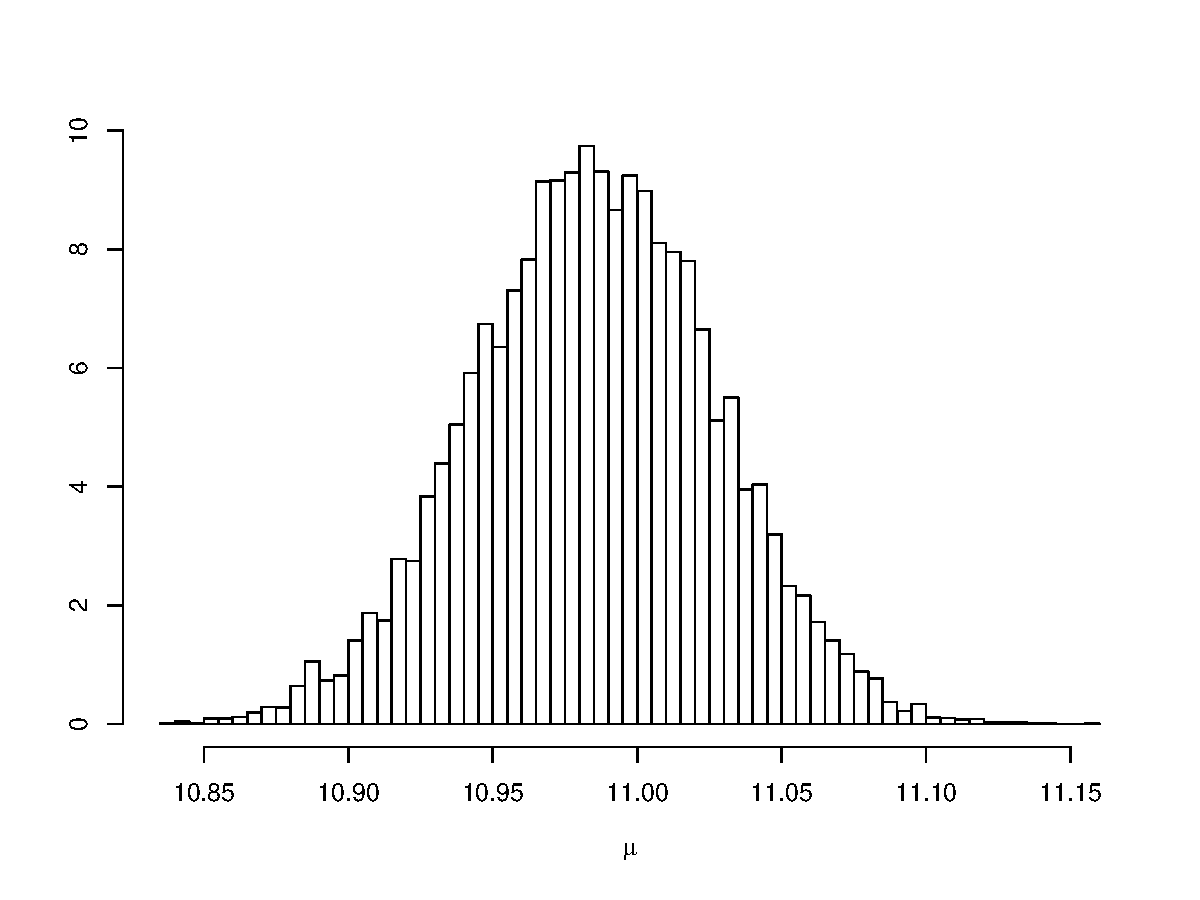
\includegraphics[scale=0.4]{figuras/mu_mh_50000.pdf}}}%
	\qquad
	\subfloat[Histograma de $\sigma^2$]{{
			\label{fig:s2_mh_50000}
			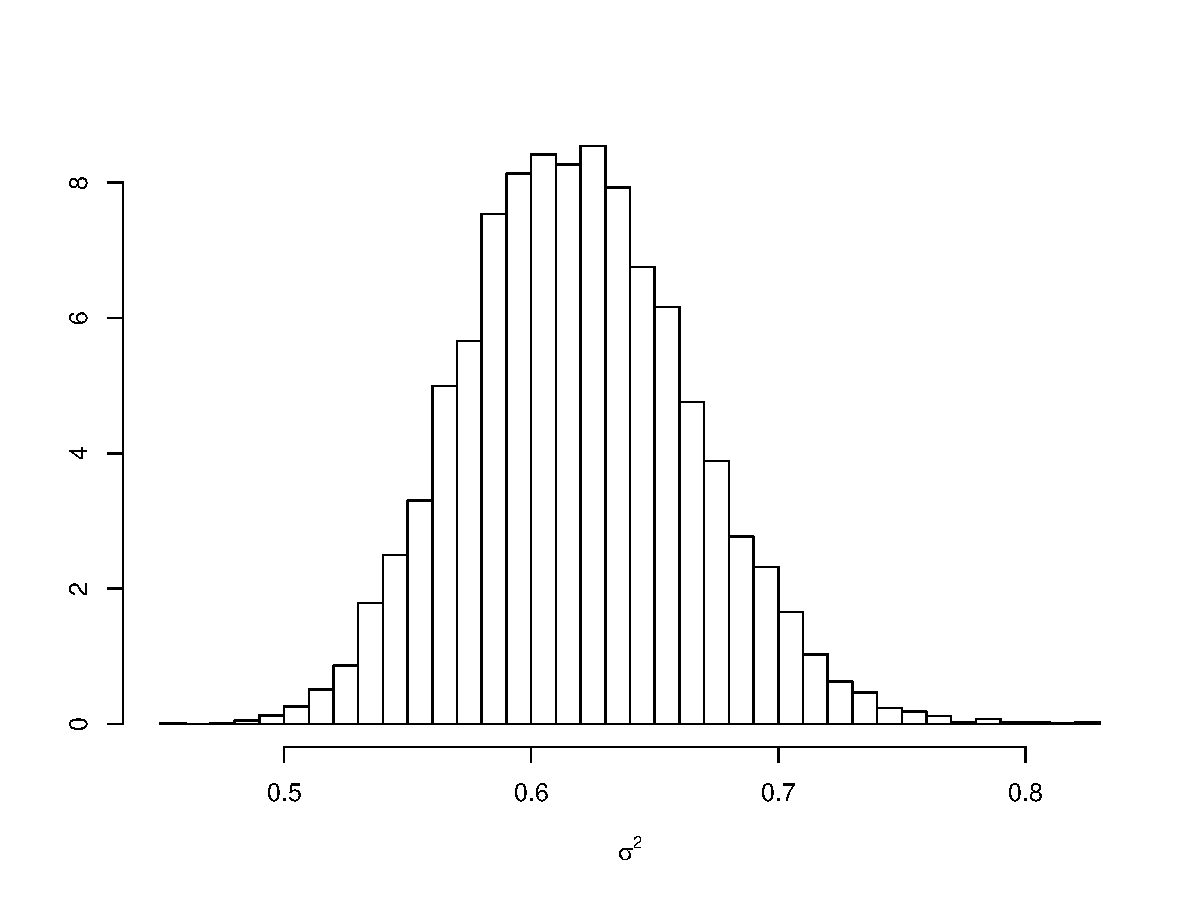
\includegraphics[scale=0.4]{figuras/s2_mh_50000.pdf}}}%
	\subfloat[Histograma de $\nu$]{{
			\label{fig:nu_mh_50000}
			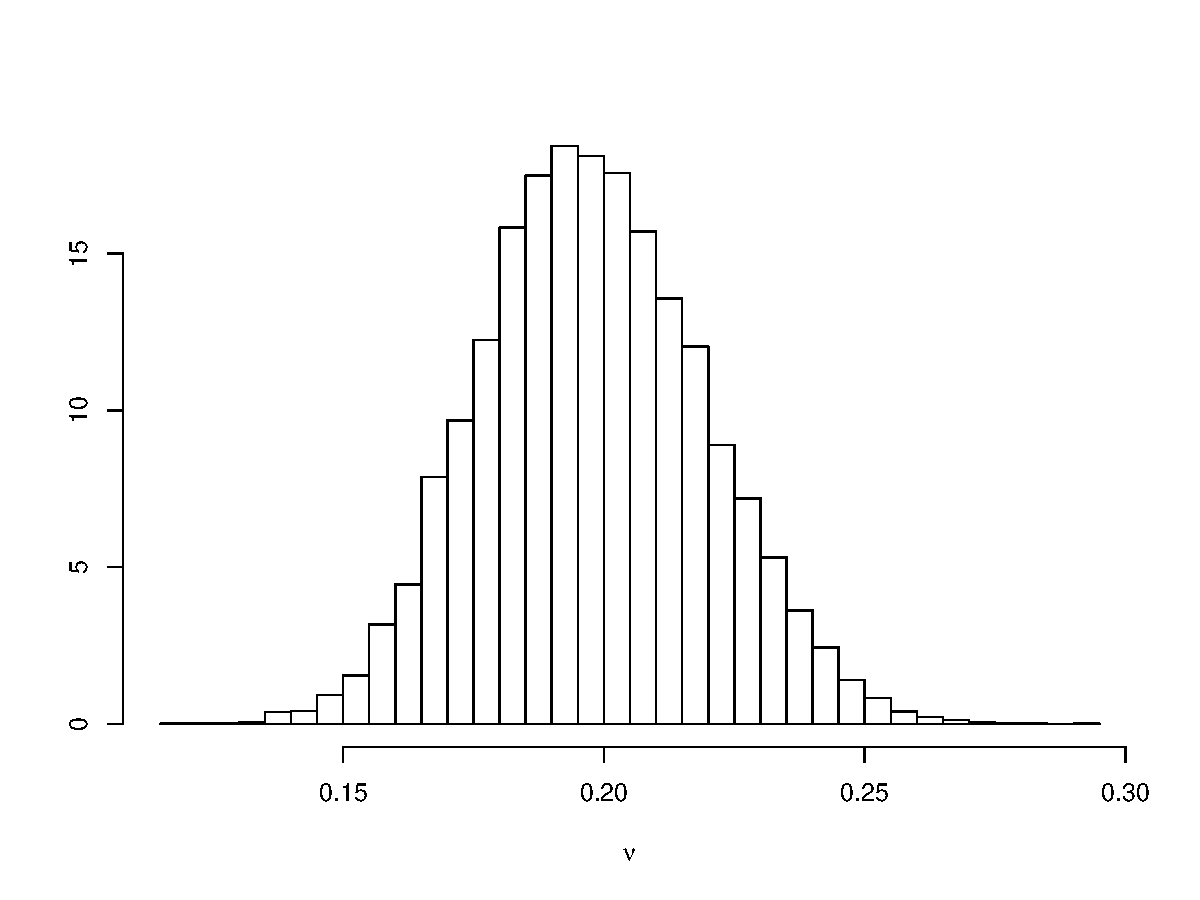
\includegraphics[scale=0.4]{figuras/nu_mh_50000.pdf}}}%
	\caption{Histograma das densidades \textit{a posteriori} marginais pela método MCMC--MH, $k = 50000$}%
\end{figure}

No presente trabalho, deseja-se amostrar os parâmetros $\mu, \sigma^2$ e $\nu$ da distribuição \textit{a posteriori} $p(\mu, \sigma^2, \nu | \bm{x})$ do modelo de mistura finita de normais com variância contaminada. O uso do algoritmo MH para cada uma das 3 cadeias correspondentes se justifica pelo fato de que: (i) em nenhum dos parâmetros é possível obter analiticamente a respectiva distribuição condicional completa, de modo que será necessário amostrar da distribuição \textit{a posteriori} conjunta, e (ii) como a distribuição \textit{a posteriori} conjunta é escrita como o produto de uma constante de proporcionalidade vezes um núcleo que depende dos parâmetros, o algoritmo MH continua válido quando se trabalha com o núcleo do lado direito de \eqref{eq:dist_post} no lugar de $p(\mu, \sigma^2, \nu | \bm{x})$. Novamente, para avaliar este núcleo, toma-se a soma do logaritmo de todas as quantidades que o compõem quando multiplicadas entre si. Assim como feito no método SIR, para a distribuição proposta $q(\cdot)$ também será escolhida uma normal trivariada $N_3(\bm{\mu}, \bm{\Sigma})$ e a mesma reparametrização para $(\mu, \sigma^2, \nu)$ será reutilizada de modo a garantir que a distribuição proposta gere adequadamente de $p(\mu, \sigma^2, \nu | \bm{x})$ pelo algoritmo MH, inclusive com os mesmos valores do vetor de médias $\bm{\mu} = (\mu, \log(\sigma^2), \log[\nu/(1-\nu)]) = (11, \log(0.64), \log[0.2/0.8])$ e da matriz de covariância $\bm{\Sigma} = \textrm{diag}\{0.0022, 0.0065, 0.0203\}$.

Para aplicar o método MCMC com algoritmo MH de modo a obter amostras \textit{a posteriori} de $\mu$, $\sigma^2$ e $\nu$, foram considerados 3 cenários: $k = \{500, 5000, 50000\}$, os mesmos do método SIR. Como no MCMC é necessário definir um estado inicial da cadeia, em geral com densidade conjunta muito baixa, escolheu-se o ponto $x_0 = (10.86, log(0.50), log(0.14/0.86))$ para inicialização do algoritmo, com logaritmo do núcleo da \textit{posteriori} avaliado em $1.760 \times 10^{-235}$, ainda numericamente não nulo pelo \textit{R}. Evidentemente, as primeiras amostras geradas não terão distribuição próxima à da limite, razão pela qual será feito um descarte (em inglês, \textit{burn-in}) de 20\% a partir dos valores iniciais. Logo, ao final se terão $400, 4000$ e $40000$ valores gerados nos cenários correspondentes. Como o vetor de valores uniformes para comparação das probabilidades de aceitação a cada passo não dependem dos valores gerados de $q$, em todos os cenários eles foram construídos fora da rotina iterativa do algoritmo MH. No final, as taxas de aceitação das amostras propostas ficaram em $45.2\%$; $40.42\%$ e $41.11\%$ para os cenários em ordem crescente de tamanho da cadeia. Nas figuras \ref{fig:mu_mh_500} a \ref{fig:nu_mh_500}; \ref{fig:mu_mh_5000} a \ref{fig:nu_mh_5000} e \ref{fig:mu_mh_50000} a \ref{fig:nu_mh_50000} são apresentados os histogramas para as amostras \textit{a posteriori} de cada parâmetro por cenário.

Para $k=500$, a aproximação da densidade não é boa para nenhum dos 3 parâmetros com as $400$ amostras restantes: há pontos extremos distantes do que seria a massa principal, especialmente para $\nu$. Além disso, há várias modas locais, indicando uma curva que está longe de ser suave. Entretanto, é possível dizer já neste cenário como é o comportamento de cada parâmetro com relação à locação, assim como no método SIR.

Para $k=5000$, a aproximação é bem mais suave e há menos \textit{outliers} quando consideradas as $4000$ amostras restantes. O número de modas locais também é reduzido em comparação ao cenário anterior, embora esta quantidade ainda seja moderada para $\sigma^2$ e alta para $\nu$. Além do comportamento com relação à locação, é possível dizer também como é o comportamento com relação à dispersão da densidade \textit{a posteriori} marginal de cada parâmetro, mas não com relação à assimetria, ao contrário do método SIR.

Para $k=50000$, os gráficos confirmam a tendência apresentada pelo cenário anterior, mas com uma suavização ainda melhor, embora não tão boa quanto no algoritmo SIR para a mesma quantidade de amostras \textit{a posteriori} geradas, mesmo com o \textit{burn-in} de 20\% das amostras. Isso se pelo fato de que o começo da cadeia é fortemente influenciada pela escolha do valor inicial mesmo com o \textit{burn-in}, mas essa influência vai diminuindo ao longo dos passos do algoritmo. Todas as distribuições são praticamente unimodais (há algumas modas locais quase imperceptíveis nos gráficos de $\mu$ e $\sigma^2$) e praticamente não há mais \textit{outliers}. Agora, é possível identificar uma leve assimetria à direita nos gráficos de $\sigma^2$ e $\nu$.

Obtidas as amostras \textit{a posteriori} marginais de cada parâmetro, para aproximar as estatísticas de média, variância, assimetria e curtose novamente serão tomadas as respectivas estimativas amostrais. Na Tabela \ref{tab3}, são apresentados os valores aproximados para tais estatísticas em cada um dos três cenários.

\begin{table}[htb]
	\caption{Estatísticas \textit{a posteriori} para $(\mu, \sigma^2, \nu)$ pelo método MCMC--MH}
	\label{tab3}
	\centering
	\begin{tabular}{cccccc}
		\toprule
		Cenário & Parâmetro & Média & Variância & Assimetria & Curtose \\
		\midrule
		$k = 500$ & $\mu$ & 10.9672 & 0.0018 & -0.3768 & 3.2193 \\
		& $\sigma^2$ & 0.6226 & 0.0020 & -0.0684 & 2.6117 \\
		& $\nu$      & 0.1957 & 0.0006 & -0.3313 & 3.2991 \\
		\midrule
		$k = 5000$ & $\mu$ & 10.9818 & 0.0019 & -0.2466 & 2.9894 \\
		& $\sigma^2$ & 0.6197 & 0.0023 & 0.2372 & 3.0057 \\
		& $\nu$      & 0.1977 & 0.0005 & 0.3878 & 3.2038 \\
		\midrule
		$k = 50000$ & $\mu$ & 10.9852 & 0.0017 & -0.0272 & 2.9451 \\
		& $\sigma^2$ & 0.6188 & 0.0021 & 0.2472 & 3.1088 \\
		& $\nu$      & 0.1978 & 0.0005 & 0.1331 & 2.8971 \\
		\bottomrule
	\end{tabular}
\end{table}

Pela Tabela \ref{tab3}, pode-se concluir que tanto a média quanto a variância \textit{a posteriori} variaram muito pouco nos três cenários, independente do parâmetro considerado. Logo, amostras \textit{a posteriori} de tamanho moderado são o suficiente para se obter uma boa aproximação destas duas estatísticas. Por outro lado, o mesmo não pode ser dito para a assimetria e curtose \textit{a posteriori}, para as quais há grandes mudanças inclusive na primeira casa decimal, mesmo de $k=5000$ para $k=50000$, assim como no método SIR (Tabela \ref{tab2}). Apesar deste fato, no método MCMC com passos MH também se pode dizer que houve uma estabilidade nas aproximações destas duas últimas estatísticas na medida em que $k$ crescia, embora com convergência mais lenta do que no método SIR.

Com relação aos valores em si, as médias \textit{a posteriori} para os 3 parâmetros ficaram muito próximas dos respectivos valores do modelo para a distribuição amostral, embora não tanto quanto no método SIR. Para as variâncias \textit{a posteriori}, todas elas foram bem pequenas, em especial para $\nu$, assim como na quadratura e no SIR. Com relação à assimetria \textit{a posteriori}, esta foi praticamente nula para $\mu$ e positiva, mas fraca, para $\sigma^2$ e $\nu$ (um pouco mais forte para a primeira, assim como na quadratura e diferente do método SIR). Por fim, as aproximações para a curtose \textit{a posteriori} foram todas bem próximas de 3 (em geral, acima deste valor), com o parâmetro $\mu$ mais próximo desse valor e $\sigma^2$ o mais afastado, a mesma conclusão na quadratura.

Por fim, no Anexo são apresentados os gráficos de convergência (traço) e de autocorrelação das 9 cadeias geradas (3 para cada cenário, correspondentes a cada parâmetro), nas figuras \ref{fig:trace_mu_mh} a \ref{fig:acf_nu_mh}. Para todos os parâmetros, podemos dizer que houve convergência para a distribuição limite, o que fica bastante evidentemente no cenário $k = 50000$. Com relação à autocorrelação, é necessário uma defasagem (em inglês, \textit{lag}) moderada, de tamanho pelo menos igual a 20, para remover a autocorrelação dentro da cadeia. Como $k$ é grande se comparado a este valor em todos os cenários, isto afetará pouco nas estimativas de variância \textit{a posteriori} para cada parâmetro.